\documentclass[handout]{beamer}
%\documentclass[presentation]{beamer}

\usecolortheme{Imperial}
 
\usepackage[utf8]{inputenc}
\usepackage[UKenglish]{babel}
\usepackage{booktabs}
\usepackage{caption}
\usepackage{subcaption}
\usepackage{graphicx}
\usepackage{amsmath}
\usepackage{amsfonts}
\usepackage{amssymb}
\usepackage{epstopdf}
%\usepackage{subfig} %this package cause an error for some reason
\usepackage{tikz}
\usetikzlibrary{patterns}
\usepackage{multirow} %to center a table cell with the multi lines cells in its row
\usepackage{schemabloc}
\usetikzlibrary{arrows,shapes,snakes,automata,backgrounds,petri}
%\usepackage[colorlinks=true, allcolors=blue]{hyperref}
\usepackage{amssymb}%for nested sets
\usepackage{tikz}%for nested sets
\usetikzlibrary{positioning}%for nested sets
\tikzset{set/.style={draw,circle,inner sep=0pt,align=center}}%for nested sets
\usepackage{pgfplots} % for processor chart
\usetikzlibrary{intersections} % for processor chart
\pgfplotsset{compat=newest}% for processor chart
\usepackage{tikzscale}% for processor chart
\usepackage{pifont}% check-mark
\newcommand{\cmark}{\ding{51}}% check-mark
\newcommand{\xmark}{\ding{55}}% check-mark
\usepackage{caption}% caption font size
\captionsetup[figure]{font=footnotesize}% caption font size
\usepackage{caption} %to remove the word figure in figures' caption
\captionsetup[figure]{labelformat=empty}% to remove the word figure in figures' caption

%%%%%%%%%%%%%%%%%%%%%%%%%%%%%%%%%%%%%%%%%%%%%%%%% COLORS %%%%%%%%%%%%%%%%%%%%%%%%%%%%%%%%%%%%%%%%
%Random Colors
\definecolor{light blue}{HTML}{bdc9e1}
\definecolor{otherbluegantt}{HTML}{67a9cf}
\definecolor{myLightGray}{RGB}{191,191,191}
\definecolor{myGray}{RGB}{160,160,160}
\definecolor{myDarkGray}{RGB}{144,144,144}
\definecolor{myDarkRed}{RGB}{167,114,115}
\definecolor{myRed}{HTML}{e41a1c}
\definecolor{myGreen}{HTML}{4daf4a}
\definecolor{myBlue}{HTML}{377eb8}
\definecolor{Gainsboro}{HTML}{DCDCDC}
\definecolor{light gray}{HTML}{BDBDBD}

\definecolor{skiastro}{HTML}{abd9e9}
\definecolor{newpoints}{HTML}{fdae61}
\definecolor{points}{HTML}{2c7bb6}

\definecolor{blue1}{HTML}{f0f9e8}
\definecolor{blue2}{HTML}{bae4bc}
\definecolor{blue3}{HTML}{7bccc4}
\definecolor{blue4}{HTML}{2b8cbe}

%sequential right (1)
\definecolor{seqr1}{HTML}{B7E6A5}
\definecolor{seqr2}{HTML}{7CCBA2}
\definecolor{seqr3}{HTML}{46AEA0}
\definecolor{seqr4}{HTML}{089099}

%Diverging (1)
\definecolor{div1}{HTML}{009392}
\definecolor{div2}{HTML}{39B185}
\definecolor{div3}{HTML}{9CCB86}
\definecolor{div4}{HTML}{E9E29C}

%Diverging (2)
\definecolor{div21}{HTML}{089099}
\definecolor{div22}{HTML}{7CCBA2}
\definecolor{div23}{HTML}{FCDE9C}
\definecolor{div24}{HTML}{F0746E}


\definecolor{light blue}{HTML}{74BBC9}
\definecolor{yellow}{HTML}{F7E967}

% complying UK date format, i.e. 1 January 2001
\usepackage{datetime}
\let\dateUKenglish\relax
\newdateformat{dateUKenglish}{\THEDAY~\monthname[\THEMONTH] \THEYEAR}

% Imperial College Logo, not to be changed!
\institute{\includegraphics[height=0.7cm]{Imperial_1_Pantone_solid.eps}}

% -----------------------------------------------------------------------------




%Information to be included in the title page:
\title{Data Analysis with Mixed-Integer Optimisation for Scheduling Royal Mail Deliveries}

\subtitle{MENG INDIVIDUAL PROJECT}

\author{Athanasios Liaskas}

\date{\today}



\begin{document}
 
\frame{\titlepage}

%%%%%%%%%%%%%%%%%%%%%%%%%%%%%%%%%%%%%%%%%%%%%%%%%%%%%%%%%%%%%%%%%%%FRAME%%%%%%%%%%%%%%%%%%%%%%%%%%%%%%%%%%%%%%%%%%%%%%%%%%%%%%%%%%%%%%%%%%%%%%%%%%%%%

\begin{frame}
	\frametitle{Problem Description}
	
	\begin{columns}[]
	    \centering
			\column{0.4875\textwidth}
			\textbf{\uline{Context of the Problem}}
			\begin{itemize}
				\item Each MC is responsible for a broad geographic region.
				\item Trips are performed by each MC's fleet of HGV vehicles.
			\end{itemize}			
		\column{0.5275\textwidth}
			\centering
\begin{figure}%
    \centering
    \scalebox{.62}{
		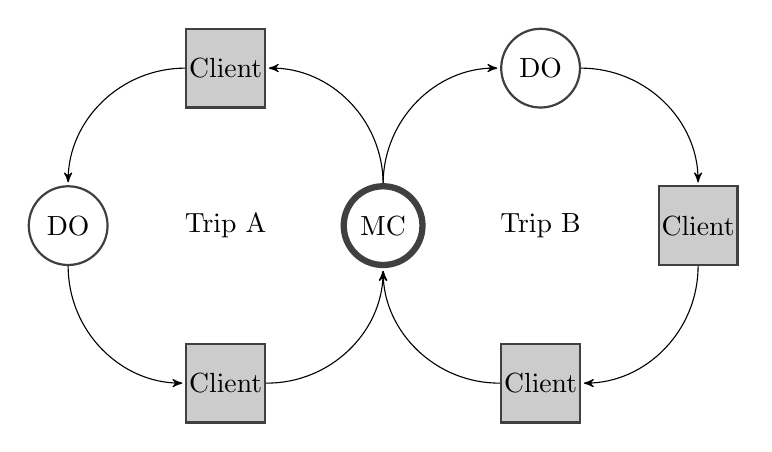
\begin{tikzpicture}[node distance=2cm,>=stealth',bend angle=45,auto,rotate=90,transform shape]%picture #1

      \tikzstyle{place}=[circle,thick,draw=black!75,fill=white!20,minimum size=10mm]
      \tikzstyle{red place}=[place,draw=red!75,fill=red!20]
      \tikzstyle{transition}=[rectangle,thick,draw=black!75,
      			  fill=black!20,minimum size=10mm]
    
      \tikzstyle{every label}=[black]
    
      \begin{scope}
        
        
        %All but clients
        \node [place,label={[rotate=-90]center:DO}] (w1)                                    {};
        \node [place, draw=white,label={[rotate=-90]center:Trip A}] (c1) [below of=w1]                      {};
        \node [place, line width=0.8mm,label={[rotate=-90]center:MC}] (s)  [below of=c1] {};
        \node [place, draw=white,label={[rotate=-90]center:Trip B}] (c2) [below of=s]                       {};
        \node [place,label={[rotate=-90]center:DO}] (w2) [right of=c2]                      {}
            edge [pre,bend right]                (s);
    
        %boxes w/ Clients
        \node [transition,label={[rotate=-90]center:Client}] (e1) [left of=c1] {}
          edge [pre,bend left]                  (w1)
          edge [post,bend right]                (s);
    
        \node [transition,label={[rotate=-90]center:Client}] (e2) [left of=c2] {}
          edge [post,bend left]                 (s);
    
        \node [transition,label={[rotate=-90]center:Client}] (l1) [right of=c1] {}
          edge [pre,bend left]                  (s)
          edge [post,bend right] node[swap] {} (w1);
    
        \node [transition,label={[rotate=-90]center:Client}] (l2) [below of=c2] {}
          edge [pre,bend right]                 (w2)
          edge [post,bend left]  node {}       (e2);
      \end{scope}

\end{tikzpicture}}%picture #1
  \label{fig:Atomic block}%
\end{figure}

	\end{columns}
	
	\begin{block}{Atomic Block Definition}
		A \textbf{single round-trip} that commences at the Exeter MC, and after stopping at various external locations concludes again at the MC.
	\end{block}
	

\vspace{\baselineskip}
\end{frame}

%%%%%%%%%%%%%%%%%%%%%%%%%%%%%%%%%%%%%%%%%%%%%%%%%%%%%%%%%%%%%%%%%%%FRAME%%%%%%%%%%%%%%%%%%%%%%%%%%%%%%%%%%%%%%%%%%%%%%%%%%%%%%%%%%%%%%%%%%%%%%%%%%%%%


\begin{frame}
	\frametitle{Breakdown of an Atomic Block}
	\vspace{\baselineskip}
\begin{figure}
    \centering
    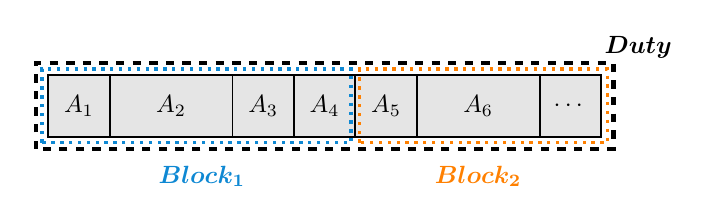
\begin{tikzpicture}[line width=.7pt,scale=0.78, every node/.style={scale=0.9}]
        %Activities
        \draw[fill=gray!20] (0,0)node[below]{} rectangle(1,1);
        %%%%%%%%%%%%%%%%%%%%%%%%%%%%%% NOTATION %%%%%%%%%%%%%%%%%%%
        %%%%%%%%%%%%%%%%%%%%%(bottomleft)             (topright)
        \draw[fill=gray!20] (1,0)node[below]{} rectangle(3,1);
        \draw[fill=gray!20] (3,0)node[below]{}rectangle(4,1);
        \draw[fill=gray!20] (4,0)node[below]{}rectangle (5,1)(2.5,1)node[below,yshift=-1.15cm, text=cyan!70!blue]{$\boldsymbol{Block_1}$};
        \draw[fill=gray!20] (5,0)node[below]{}rectangle (6,1);
        \draw[fill=gray!20] (6,0)node[below]{}rectangle (8,1);
        \draw[fill=gray!20] (8,0)node[below]{}rectangle (9,1)(7,1)node[below,yshift=-1.15cm, text=orange]{$\boldsymbol{Block_2}$}(9.605,0.75)node[below,yshift=0.9cm]{$\boldsymbol{Duty}$};
        %Blocks
        %\draw[fill=none, double=gray!40,double distance =1pt] (-0.1,-0.1)node[below]{} rectangle(4.93,1.1);
        %\draw[fill=none, double=red,double distance =1pt] (5.07,-0.1)node[below]{} rectangle(9.1,1.1);
        \draw[fill=none,very thick,dotted,draw=cyan!70!blue] (-0.1,-0.1)node[below]{} rectangle(4.93,1.1);
        \draw[fill=none,very thick,dotted,draw=orange] (5.07,-0.1)node[below]{} rectangle(9.1,1.1);
        %Duty
        \draw[fill=none,ultra thick,dashed] (-0.2,-0.2)node[below]{} rectangle(9.2,1.2);
        
        \path (0.5,.5)node{$A_1$} (2,.5)node{$A_2$} (3.5,.5)node{$A_3$} (4.5,.5)node{$A_4$} (5.5,.5)node{$A_5$} (7,.5)node{$A_6$} (8.5,.5)node{$\dotsi$};
        %%%%%%%(width of label, height)
        \end{tikzpicture}
    \caption{Structure of a driver's Duty: $Activities \: (A_{i}$), inside $Atomic \: Blocks$ which themselves create a $Duty$.}
    \label{fig:Duty-Block-Activity}
\end{figure}

\vspace{\baselineskip}
\end{frame}


%%%%%%%%%%%%%%%%%%%%%%%%%%%%%%%%%%%%%%%%%%%%%%%%%%%%%%%%%%%%%%%%%%%FRAME%%%%%%%%%%%%%%%%%%%%%%%%%%%%%%%%%%%%%%%%%%%%%%%%%%%%%%%%%%%%%%%%%%%%%%%%%%%%%

\begin{frame}
	\frametitle{What is an Activity?}
	\vspace{\baselineskip}
	\begin{block}{Types of \textit{Activities} featured in the dataset}
	    The set of activities signifying the \textit{task by task} actions performed by drivers, as observed in the data exploration.
	\end{block}
	
	
	\begin{table}[ht]
\small
    \centering 
    \begin{tabular}{|l|l|}
        \hline
        \multicolumn{1}{|c|}{ \textbf{Activity}} & \multicolumn{1}{|c|}{ \textbf{Description}} \\
        \hline
        Start/End & The \textit{beginning}, and \textit{end} of a duty. \\
        \hline
        Travel & A \textit{travel leg} between locations. \\ 
        \hline
        Load/Unload  & \textit{Loading} and \textit{offloading} of mail units.\\ 
        \hline
        Meal Relief & A \textit{meal-allowance} break. \\ 
        \hline
        Distribution/Processing & Non-essential administrative tasks. \\     
        \hline
        Park Vehicle  & \textit{Parking} of HGV at end of duty.\\ 
        \hline
        Check & Scheduled \textit{servicing} of HGV. \\ 
        \hline
        Clean & Scheduled \textit{cleaning} of HGV. \\ 
        \hline
    \end{tabular}
    \medbreak
    \label{table:Activity List}
\end{table}
\vspace{\baselineskip}
\end{frame}


%%%%%%%%%%%%%%%%%%%%%%%%%%%%%%%%%%%%%%%%%%%%%%%%%%%%%%%%%%%%%%%%%%%FRAME%%%%%%%%%%%%%%%%%%%%%%%%%%%%%%%%%%%%%%%%%%%%%%%%%%%%%%%%%%%%%%%%%%%%%%%%%%%%%

\begin{frame}
	\frametitle{High-level Overview}
	\begin{columns}[]
		\column{0.0125\textwidth}
		\column{0.4875\textwidth}
			\centering
			\begin{figure}
			\captionsetup{justification=centering}
                \centering
            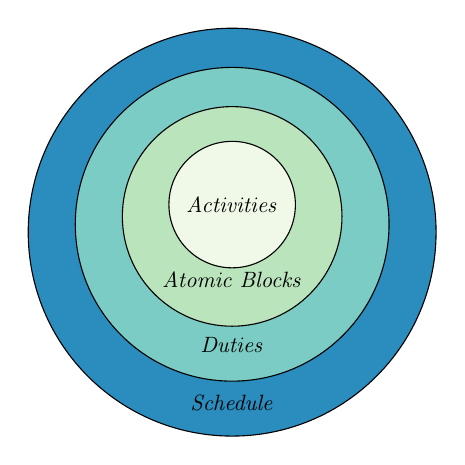
\begin{tikzpicture}[scale=0.5, every node/.style={scale=0.8}]
            \node[set,fill=blue4,text width=6.5cm,label={[below=130pt of rea,text opacity=1]\textit{Schedule}}] 
                (nat) at (0,-0.7)  (rea) {};
            \node[set,fill=blue3,text width=5cm,label={[below=95pt of rea,text opacity=1]\textit{Duties}}] 
              (nat) at (0,-0.5)  (rea) {};
            \node[set,fill=blue2,text width=3.5cm,label={[below=57pt of int]\textit{Atomic Blocks}}] 
              (int) at (0,-0.3)  {};
            \node[set,fill=blue1,text width=2cm] (nat) at (0,0) {\textit{Activities}};
            \end{tikzpicture}%picture #1
                    \footnotesize{ \caption{The \textit{duty} assigned to each driver is a collection of \textit{blocks}, which themselves contain \textit{activities}.}}
                    \label{fig:Nested-set}
			\end{figure}
		\column{0.4875\textwidth}
			\textbf{Key Data Points}
			\begin{itemize}
				\item \footnotesize{\underline{Activity:} Intervals of activity enclosed inside an \texttt{Atomic Block}.}
				\item \underline{Atomic Block:} A round-trip starting and concluding at the MC.
				\item \underline{Duty:} The total time that a driver works for, in a day.
			\end{itemize}			
		\column{0.0125\textwidth}
	\end{columns}
\end{frame}


%%%%%%%%%%%%%%%%%%%%%%%%%%%%%%%%%%%%%%%%%%%%%%%%%%%%%%%%%%%%%%%%%%%FRAME%%%%%%%%%%%%%%%%%%%%%%%%%%%%%%%%%%%%%%%%%%%%%%%%%%%%%%%%%%%%%%%%%%%%%%%%%%%%%

\begin{frame}
	\frametitle{Royal Mail Historical Schedules}
	\vspace{\baselineskip}
	
    \begin{block}{What is a Schedule?}
		The set of all the \textbf{duties} assigned to each HGV driver for a day of the week.
	\end{block}
	
	\begin{columns}[b]
		\column{0.0125\textwidth}
		\column{0.3975\textwidth}
			\centering
		    \begin{figure}
			   \includegraphics[width=\textwidth]{Images/Appendix-Start-wave.png} \
			 \end{figure}
		\column{0.3975\textwidth}
			\centering
	        \begin{figure}
			    \includegraphics[width=\textwidth]{Images/schedule.PNG} \
			\end{figure}
		\column{0.0125\textwidth}
	\end{columns}

	
\vspace{\baselineskip}
\vspace{\baselineskip}
\vspace{\baselineskip}
\vspace{\baselineskip}
\end{frame}

%%%%%%%%%%%%%%%%%%%%%%%%%%%%%%%%%%%%%%%%%%%%%%%%%%%%%%%%%%%%%%%%%%%FRAME%%%%%%%%%%%%%%%%%%%%%%%%%%%%%%%%%%%%%%%%%%%%%%%%%%%%%%%%%%%%%%%%%%%%%%%%%%%%%

\begin{frame}
	\frametitle{Evaluation of Historical Schedules}
	\vspace{\baselineskip}
	
	\begin{columns}[]
			\column{0.4875\textwidth}
			\textbf{Motivation for Sensitivity Analysis}
			\begin{itemize}
				\item How good are the historical schedules, and can they be improved?
				\item Our goal is to propose schedules with favourable characteristics. 
			\end{itemize}			
		\column{0.0125\textwidth}
		\column{0.0125\textwidth}
		\column{0.4875\textwidth}
			\centering
            \begin{figure}
				\includegraphics[width=\textwidth]{Images/sketo.png}
				% remove the 'draft' keyword, when replacing with final figure!
			\end{figure}

	\end{columns}
	

	

\vspace{\baselineskip}
\end{frame}

%%%%%%%%%%%%%%%%%%%%%%%%%%%%%%%%%%%%%%%%%%%%%%%%%%%%%%%%%%%%%%%%%%%FRAME%%%%%%%%%%%%%%%%%%%%%%%%%%%%%%%%%%%%%%%%%%%%%%%%%%%%%%%%%%%%%%%%%%%%%%%%%%%%%

\begin{frame}
	\frametitle{Simplifying Assumptions}
	\vspace{\baselineskip}
	\begin{table}[h]
		\centering
		\begin{tabular}{p{0.1\textwidth} p{0.8\textwidth}} 
			\toprule
			\multicolumn{2}{p{0.8\textwidth}}{\textbf{Key Simplifications}} \\
			\midrule
			\textbf{(1)}       & We consider a \textbf{duty} as a \textit{machine} and a \textbf{block} as a \textit{job}, freely assigning blocks to duties. \\
			\textbf{(2)}       & The \textbf{duration} of a \textbf{block} stays \textbf{constant}, irrespective of the timing of its occurrence.\\
			\textbf{(3)}  & The \textbf{routes} are \textbf{fixed}, and we \textbf{maintain} the \textbf{order} with which we visit external locations.\\
			\bottomrule
		\end{tabular} 
	\end{table}


\end{frame}

%%%%%%%%%%%%%%%%%%%%%%%%%%%%%%%%%%%%%%%%%%%%%%%%%%%%%%%%%%%%%%%%%%%FRAME%%%%%%%%%%%%%%%%%%%%%%%%%%%%%%%%%%%%%%%%%%%%%%%%%%%%%%%%%%%%%%%%%%%%%%%%%%%%%

\begin{frame}

	\frametitle{Load Balancing}
	
\vspace{\baselineskip}
			
		    \textbf{Model Description}
		    
			\begin{itemize}
				\small{\item \underline{Objective:} find a more \textbf{balanced schedule} in terms of \textbf{duty length}.}
				\item We minimise the \textbf{maximum length of a duty}.
				\item We execute all blocks featured in the historical schedule.
				\item Each driver executes at most one block per unit of time.
			\end{itemize}	
			
			\vspace{\baselineskip}
			\centering
			\scalebox{0.7}{
			\begin{equation*}
                \begin{aligned}
                &\text{minimize}
                %& & y_{i}  \\ %\todo{why y and and not yi}
                & & y  \\ 
                & \text{subject to}
                % & & y_{i} = \sum _{j=1}^n x_{i,j}p_{j}  \;\;\; &\forall \; i \in D\tag{1}\\   
                & & y \geq \sum _{j=1}^n x_{i,j}p_{j}  \;\;\; &\forall \; i \in D\\   
                & & &\sum _{i=1}^m x_{i,j} = 1 \;\;\; &\forall \; j \in B\\
                % & & &\sum _{j=1}^n x_{i,j}p_{j} \leq f_{i}-s_{i} \;\;\; &\forall \; i \in D\\ %{\color{red} we deleted the constraint that involves the length of duty being less than end-start.}
                & & & y\geq 0  \\
                & & & x_{i,j} \in  \{ 0,1 \} \;\;\; &\forall \; j \in B, \; i \in D\\
                \end{aligned}
            \end{equation*}}

\end{frame}

%%%%%%%%%%%%%%%%%%%%%%%%%%%%%%%%%%%%%%%%%%%%%%%%%%%%%%%%%%%%%%%%%%%FRAME%%%%%%%%%%%%%%%%%%%%%%%%%%%%%%%%%%%%%%%%%%%%%%%%%%%%%%%%%%%%%%%%%%%%%%%%%%%%%

\begin{frame}
\label{slide: makespan Scheduling}
	\frametitle{Numerical Results}


	\begin{columns}[]
		\column{0.0125\textwidth}
		\column{0.585\textwidth}
			\centering
	   	\begin{figure}%
        \centering
        \includegraphics[width=0.8\textwidth]{Images/1-D1M1.png}
        %\end{center}}%end of picture #2
        %\caption{Illustrations of curves indicating our results.}%
        \label{fig:1-D1M1}%
    \end{figure} 
		\column{0.4\textwidth}
    	\scalebox{0.7}{
    \begin{table}[h]
    \small
    \centering 
    \begin{tabular}{c|c}
            \multicolumn{2}{c}{\textbf{(\%) Reduction }} \\
            \hline
            \textbf{Makespan} & \textbf{Maximum Difference} \\
            \hline
             28\% & 72\% \\
    
    \end{tabular}
    
    \end{table}
    }
    \column{0.10125\textwidth}
	\end{columns}

        
        \begin{block}{Results Interpretation}
		A more \textbf{balanced} schedule. We redistributed the workload to reduce the amount of overtime that drivers need to perform.
	\end{block}

    
\end{frame}

%%%%%%%%%%%%%%%%%%%%%%%%%%%%%%%%%%%%%%%%%%%%%%%%%%%%%%%%%%%%%%%%%%%FRAME%%%%%%%%%%%%%%%%%%%%%%%%%%%%%%%%%%%%%%%%%%%%%%%%%%%%%%%%%%%%%%%%%%%%%%%%%%%%%

\begin{frame}
	\frametitle{Number of Duties vs Maximum Duty Length}
	
			    \vspace{\baselineskip}
		    \textbf{Model Description}
			\begin{itemize}
                \item \small{We fix an upper threshold of duty length \textbf{$L$} and execute all blocks while \textbf{\textit{minimising the amount of duties.}}}
				\item We vary \textbf{$L$} and conduct a Sensitivity Analysis to determine the minimum number of duties that give us a feasible schedule.
			\end{itemize}	
	
\vspace{\baselineskip}
			\centering
			\scalebox{0.7}{
			\begin{equation*}
                \begin{aligned}
                &\text{minimize}
                & & \sum _{i=1}^m y_{i}  \\
                & \text{subject to}
                & & y_{i} \geq x_{i,j}  \;\;\; &\forall \; i \in D,\; j \in B\\   
                & & &\sum _{i=1}^m x_{i,j} = 1 \;\;\; &\forall \; j \in B\\
                %& & &\sum _{j=1}^n x_{i,j}p_{j} \leq f_{i}-s_{i} \;\;\; &\forall \; i \in D\\
                & & &\sum _{j=1}^n x_{i,j}p_{j} \leq L \;\;\; &\forall \; i \in D\\
                & & & y\geq 0  \\
                & & & x_{i,j} \in  \{ 0,1 \} \;\;\; &\forall \; j \in B, \; i \in D\\
                \end{aligned}
            \end{equation*}}
		    


\end{frame}


%%%%%%%%%%%%%%%%%%%%%%%%%%%%%%%%%%%%%%%%%%%%%%%%%%%%%%%%%%%%%%%%%%%FRAME%%%%%%%%%%%%%%%%%%%%%%%%%%%%%%%%%%%%%%%%%%%%%%%%%%%%%%%%%%%%%%%%%%%%%%%%%%%%%

\begin{frame}
	\frametitle{Numerical Results}
	\vspace{\baselineskip}
	\begin{figure}%
        \centering
        \includegraphics[width=0.4\linewidth]{Images/1-D1M2.png}
        %\end{center}}%end of picture #2
        %\caption{Illustrations of curves indicating our results.}%
        \label{fig:1-D1M1}%
    \end{figure}
    
        \begin{block}{Results Interpretation}
		There is a trade-off between the maximum duty length and the number of duties. It is possible to schedule \textbf{all blocks} with around \textbf{30\% fewer duties.} 
	\end{block}
    	\vspace{\baselineskip}
    	\vspace{\baselineskip}
\end{frame}

%%%%%%%%%%%%%%%%%%%%%%%%%%%%%%%%%%%%%%%%%%%%%%%%%%%%%%%%%%%%%%%%%%%FRAME%%%%%%%%%%%%%%%%%%%%%%%%%%%%%%%%%%%%%%%%%%%%%%%%%%%%%%%%%%%%%%%%%%%%%%%%%%%%%

\begin{frame}
	\frametitle{Number of Blocks with Limited Driver Time}
	\vspace{\baselineskip}
	
			    \textbf{Model Description}
			\begin{itemize}
                \item \small{Minimise the maximum duty $L$ and determine the \textbf{\textit{maximum number of blocks}} that can \textbf{\textit{still be completed.}}}
				\item We preserve the duties at the historical level of 183 duties.
				\item We conduct a Sensitivity Analysis by varying $L$ to determine the maximum number of blocks that can be processed for each $L$.
			\end{itemize}	
	
\vspace{\baselineskip}
			\centering
			\scalebox{0.7}{
			\begin{equation*}
                \begin{aligned}
                &\text{maximize}
                & & \sum _{i=1}^m x_{i,j}  \\
                & \text{subject to}
                & &\sum _{i=1}^m x_{i,j} \leq 1 \;\;\; &\forall \; j \in B\\
                & & &\sum _{j=1}^n x_{i,j}p_{j} \leq L \;\;\; &\forall \; i \in D\\
                & & & y\geq 0  \\
                & & & x_{i,j} \in  \{ 0,1 \} \;\;\; &\forall \; j \in B, \; i \in D\\
                \end{aligned}
            \end{equation*}}
		    
		    \vspace{\baselineskip}


\end{frame}

%%%%%%%%%%%%%%%%%%%%%%%%%%%%%%%%%%%%%%%%%%%%%%%%%%%%%%%%%%%%%%%%%%%FRAME%%%%%%%%%%%%%%%%%%%%%%%%%%%%%%%%%%%%%%%%%%%%%%%%%%%%%%%%%%%%%%%%%%%%%%%%%%%%%

\begin{frame}
	\frametitle{Numerical Results}
	\vspace{\baselineskip}
	\begin{figure}%
        \centering
        \includegraphics[width=0.4\linewidth]{Images/1-D1M3.png}
        %\end{center}}%end of picture #2
        %\caption{Illustrations of curves indicating our results.}%
        \label{fig:1-D1M1}%
    \end{figure}
    
        \begin{block}{Results Interpretation}
		Reducing the maximum time a driver works for by \textbf{25\%} only reduces the number of blocks that can be processed by \textbf{10\%}.
	\end{block}
    	\vspace{\baselineskip}
    	\vspace{\baselineskip}
\end{frame}

%%%%%%%%%%%%%%%%%%%%%%%%%%%%%%%%%%%%%%%%%%%%%%%%%%%%%%%%%%%%%%%%%%%FRAME%%%%%%%%%%%%%%%%%%%%%%%%%%%%%%%%%%%%%%%%%%%%%%%%%%%%%%%%%%%%%%%%%%%%%%%%%%%%%

\begin{frame}
	\frametitle{Eliminating Redundant Activities}
	\vspace{\baselineskip}
	
	\begin{block}{What is \textbf{\textit{useful}} time?}
	 We classify the activities as \textbf{useful} or \textbf{not} to signify which activities must be maintained when minimising \textit{non-useful} time.
	\end{block}
	
	\begin{table}[ht]
    \small
    \centering 
    \begin{tabular}{|c|c|}
        \hline
        \textbf{Activity} & Useful Time \\
        \hline
        Start/End & \cmark \\
        \hline
        Travel & \cmark\\ 
        \hline
        Load/Unload & \cmark\\ 
        \hline
        Meal Relief & \cmark\\ 
        \hline
        Distribution/Processing & \xmark\\     
        \hline
        Park Vehicle & \xmark\\ 
        \hline
        Check & \xmark\\ 
        \hline
        Clean & \xmark\\ 
        \hline
    \end{tabular}
    \medbreak
    \caption{List of \textit{useful} or \textit{not} activities.}
    \label{table:Useful time}
\end{table}
    	\vspace{\baselineskip}
    	\vspace{\baselineskip}
\end{frame}


%%%%%%%%%%%%%%%%%%%%%%%%%%%%%%%%%%%%%%%%%%%%%%%%%%%%%%%%%%%%%%%%%%%FRAME%%%%%%%%%%%%%%%%%%%%%%%%%%%%%%%%%%%%%%%%%%%%%%%%%%%%%%%%%%%%%%%%%%%%%%%%%%%%%

\begin{frame}
	\frametitle{Redefining the Problem}
	\vspace{\baselineskip}
	
	\begin{block}{Actions Taken}
		Artificially created more space for optimisation in the data by deleting activities that we classified as \textbf{non-useful working time}. 
	\end{block}
	
	\begin{columns}[]
		\column{0.0125\textwidth}
		\column{0.585\textwidth}
			\centering
	   	\begin{figure}%
        \centering
        \includegraphics[width=0.7\textwidth]{Images/1-D2M1.png}
        %\end{center}}%end of picture #2
        %\caption{Illustrations of curves indicating our results.}%
        \label{fig:1-D2M1}%
    \end{figure} 
		\column{0.5\textwidth}
    	\scalebox{0.6}{
    \begin{table}[h]
    \small
    \centering 
    \begin{tabular}{c|c|c}
            \multicolumn{3}{c}{\textbf{(\%) Reduction }} \\
            \hline
            \textbf{Schedule} & \textbf{Makespan} & \textbf{Maximum Difference} \\
            \hline
            Historical & 28\% & 72\% \\
            \hline
            Redefined & 36\% & 78\% \\
    \end{tabular}
    \end{table}
    }
    \column{0.1025\textwidth}
	\end{columns}
    
\end{frame}




%%%%%%%%%%%%%%%%%%%%%%%%%%%%%%%%%%%%%%%%%%%%%%%%%%%%%%%%%%%%%%%%%%%FRAME%%%%%%%%%%%%%%%%%%%%%%%%%%%%%%%%%%%%%%%%%%%%%%%%%%%%%%%%%%%%%%%%%%%%%%%%%%%%%

\begin{frame}
	\frametitle{Redefined Sensitivity Analysis}
	\begin{figure}%
        \centering
        \subfloat[Number of duties required as a function of the Maximum Duty Length (in 30min intervals), up to 24 hours per duty.]{%\begin{center}
        \includegraphics[width=0.4\linewidth]{Images/1-D2M2.png}
        }%\end{center}}%picture #1
        \qquad
        %picture #2
        \centering
        \subfloat[Number of blocks processed as a function of the Maximum Duty Length (in 30min intervals), up to the historical average duty length.]{%\begin{center}
        \includegraphics[width=0.4\linewidth]{Images/1-D2M3.png}
        }%\end{center}}%end of picture #2
        %\caption{Results of sensitivity analysis investigating the effects of \texttt{maximum duty length}.}%
        \label{fig:1-D2M2}%
    \end{figure}
\end{frame}

%%%%%%%%%%%%%%%%%%%%%%%%%%%%%%%%%%%%%%%%%%%%%%%%%%%%%%%%%%%%%%%%%%%FRAME%%%%%%%%%%%%%%%%%%%%%%%%%%%%%%%%%%%%%%%%%%%%%%%%%%%%%%%%%%%%%%%%%%%%%%%%%%%%%

\begin{frame}
	\frametitle{Concluding Remarks}
	\vspace{\baselineskip}
	\begin{table}[h]
		\centering
		\begin{tabular}{p{0.1\textwidth} p{0.8\textwidth}} 
			\toprule
			\multicolumn{2}{p{0.8\textwidth}}{\textbf{Future Directions}} \\
			\midrule
			\textbf{(1)}       & Schedules that satisfy the \textbf{Meal-Relief} constraint enforced by EU regulations. \\

			\textbf{(2)}       & Incorporating Deadline Constraints. \\
			\textbf{(3)}       & Investigating the \textit{VRP} aspect of the problem. \\
			\textbf{(4)}       & Study the effect of Ellipsoidal Uncertainty Sets. \\
			\bottomrule
		\end{tabular} 
	\end{table}


\end{frame}
 
 %%%%%%%%%%%%%%%%%%%%%%%%%%%%%%%%%%%%%%%%%%%%%%%%%%%%%%%%%%%%%%%%%%%FRAME%%%%%%%%%%%%%%%%%%%%%%%%%%%%%%%%%%%%%%%%%%%%%%%%%%%%%%%%%%%%%%%%%%%%%%%%%%%%%

\begin{frame}
	\frametitle{Appendix - Departure Waves Scheduling}
	\vspace{\baselineskip}
\begin{figure}
\minipage{0.32\textwidth}
\subfloat[Morning]{%\begin{center}
  \includegraphics[width=\linewidth]{Images/morning.png}}
\endminipage\hfill
\minipage{0.32\textwidth}
\subfloat[Afternoon]{%\begin{center}
  \includegraphics[width=\linewidth]{Images/afternoon.png}}
  
\endminipage\hfill
\minipage{0.32\textwidth}%
\subfloat[Night]{%\begin{center}
  \includegraphics[width=\linewidth]{Images/night.png}}
 
\endminipage

\end{figure}
    
        \begin{block}{Results Interpretation}
		Optimising the problem in \textit{wave sub-instances} generates schedules with an \textbf{08:25} makespan similar to the results seen in slide \ref{slide: makespan Scheduling}.
	\end{block}
    	\vspace{\baselineskip}
    	\vspace{\baselineskip}
\end{frame}

 %%%%%%%%%%%%%%%%%%%%%%%%%%%%%%%%%%%%%%%%%%%%%%%%%%%%%%%%%%%%%%%%%%%FRAME%%%%%%%%%%%%%%%%%%%%%%%%%%%%%%%%%%%%%%%%%%%%%%%%%%%%%%%%%%%%%%%%%%%%%%%%%%%%%

\begin{frame}

	\frametitle{Appendix - Pre-emptive Load Balancing}
	
\vspace{\baselineskip}
			
		    \textbf{Model Description}
		    
			\begin{itemize}
				\small{\item \underline{Objective:} find the \textbf{theoretical optimal schedule} wrt. \textbf{duty length}.}
				\item We minimise the \textbf{maximum length of a duty}.
				\item We execute all blocks featured in the historical schedule.
				\item Each driver executes at most one activity per unit of time.
			\end{itemize}	
			
			\vspace{\baselineskip}
			\centering
			\scalebox{0.7}{
\begin{equation*}
\label{equation: Makespan preemptive}
\begin{aligned}
&\text{minimise}
%& & y_{i}  \\ %\todo{why y and and not yi}
& & y  \\ 
& \text{subject to}
% & & y_{i} = \sum _{j=1}^n x_{i,j}p_{j}  \;\;\; &\forall \; i \in D\tag{1}\\   
& & y\geq \sum _{j=1}^n x_{i,j}  \;\;\; &\forall \; i \in D\\   
& & &\sum _{i=1}^m x_{i,j} = p_j \;\;\; &\forall \; j \in B\\
& & &y \geq \sum _{i=1}^m x_{i,j}  \;\;\; &\forall \; j \in B\\
% & & &\sum _{j=1}^n x_{i,j}p_{j} \leq f_{i}-s_{i} \;\;\; &\forall \; i \in D\\ %{\color{red} we deleted the constraint that involves the length of duty being less than end-start.}
& & & y,x_{i,j}\geq 0  \\
\end{aligned}
\end{equation*}}

\end{frame}
 
 %%%%%%%%%%%%%%%%%%%%%%%%%%%%%%%%%%%%%%%%%%%%%%%%%%%%%%%%%%%%%%%%%%%FRAME%%%%%%%%%%%%%%%%%%%%%%%%%%%%%%%%%%%%%%%%%%%%%%%%%%%%%%%%%%%%%%%%%%%%%%%%%%%%%

\begin{frame}
	\frametitle{Appendix - Numerical Results}

\vspace{\baselineskip}
\vspace{\baselineskip}

	\begin{columns}[]
		\column{0.0125\textwidth}
		\column{0.4875\textwidth}
			\centering
			\scalebox{0.85}{
    \begin{table}[h]
    \small
    \centering 
    \begin{tabular}{c|c}
            \multicolumn{2}{c}{\textbf{Historical}} \\
            \hline
            \textbf{Makespan} & \textbf{Optimality Gap} \\
            \hline
             08:05 & 3.1\% \\
    \end{tabular}
    \end{table}}
		\column{0.4875\textwidth}
    	\scalebox{0.85}{
    \begin{table}[h]
    \small
    \centering 
    \begin{tabular}{c|c}
            \multicolumn{2}{c}{\textbf{Redefined}} \\
            \hline
            \textbf{Makespan} & \textbf{Optimality Gap} \\
            \hline
             06:32 & 6.6\% \\
    \end{tabular}
    \end{table}
    }
    \column{0.0125\textwidth}
	\end{columns}

\vspace{\baselineskip}
\vspace{\baselineskip}
\vspace{\baselineskip}
        
        \begin{block}{Results Interpretation}
		We achieve a lower-bound with respect to the maximum duty length observed in the \textbf{theoretical optimal schedules}. They are merely theoretical limits that are practically unrealisable.
	\end{block}

    
\end{frame}

 %%%%%%%%%%%%%%%%%%%%%%%%%%%%%%%%%%%%%%%%%%%%%%%%%%%%%%%%%%%%%%%%%%%FRAME%%%%%%%%%%%%%%%%%%%%%%%%%%%%%%%%%%%%%%%%%%%%%%%%%%%%%%%%%%%%%%%%%%%%%%%%%%%%%

\begin{frame}
	\frametitle{Appendix - Glossary}

These terms are used interchangeably throughout the dissertation, to not tire the reader by using the same term repeatedly.

\begin{itemize}
\small
    \item Timetable = Schedule = Itinerary
    \item Duty = Shift 
    \item Break = Meal-Relief
    \item HGV = Heavy Goods Vehicles = 7.5 tonne lorries
    \item HGV Driver = Employee
    \item Model = Formulation 
    \item Maximum Difference\footnote{Stein C. et al. Scheduling When You Do Not Know the Number of Machines.} = Measure of the difference in the distribution of load between the heaviest and least loaded duties.
\end{itemize}

    
\end{frame}
 
\end{document}

